%	-------------------------------------------------------------------------------
% 
%
%
%		2022.07.31.일 첫 작성
%
%		불교  사성제
%
%
%
%
%	-------------------------------------------------------------------------------

	\documentclass[12pt, a4paper, oneside]{book}
%	\documentclass[12pt, a4paper, landscape, oneside]{book}

		% --------------------------------- 페이지 스타일 지정
		\usepackage{geometry}
%		\geometry{landscape=true	}
		\geometry{top 		=10em}
		\geometry{bottom		=10em}
		\geometry{left		=8em}
		\geometry{right		=8em}
		\geometry{headheight	=4em} % 머리말 설치 높이
		\geometry{headsep		=2em} % 머리말의 본문과의 띠우기 크기
		\geometry{footskip		=4em} % 꼬리말의 본문과의 띠우기 크기
% 		\geometry{showframe}
	
%		paperwidth 	= left + width + right (1)
%		paperheight 	= top + height + bottom (2)
%		width 		= textwidth (+ marginparsep + marginparwidth) (3)
%		height 		= textheight (+ headheight + headsep + footskip) (4)



		%	===================================================================
		%	package
		%	===================================================================
%			\usepackage[hangul]{kotex}				% 한글 사용
			\usepackage{kotex}						% 한글 사용
			\usepackage[unicode]{hyperref}			% 한글 하이퍼링크 사용
			\usepackage{amssymb,amsfonts,amsmath}	% 수학 수식 사용

			\usepackage{scrextend}					% 
		
			\usepackage{enumerate}			%
			\usepackage{enumitem}			%
			\usepackage{tablists}			%	수학문제의 보기 등을 표현하는데 사용
										%	tabenum


		% ------------------------------ table 
			\usepackage{longtable}			%
			\usepackage{tabularx}			%

			\usepackage{setspace}			%
			\usepackage{booktabs}			% table
			\usepackage{color}				%
			\usepackage{multirow}			%
			\usepackage{boxedminipage}		% 미니 페이지
			\usepackage[pdftex]{graphicx}	% 그림 사용
			\usepackage[final]{pdfpages}	% pdf 사용
			\usepackage{framed}			% pdf 사용
			
			\usepackage{fix-cm}	
			\usepackage[english]{babel}
	
			\usepackage{tikz}%
			\usetikzlibrary{arrows,positioning,shapes}
			%\usetikzlibrary{positioning}
			

		% --------------------------------- 	page
			\usepackage{afterpage}			% 다음페이지가 나온면 어떻게 하라는 명령 정의 패키지
%			\usepackage{fullpage}			% 잘못 사용하면 다 흐트러짐 주의해서 사용
%			\usepackage{pdflscape}			% 
			\usepackage{lscape}			%	 


			\usepackage{blindtext}
	
		% --------------------------------- font 사용
			\usepackage{pifont}				%
			\usepackage{textcomp}
			\usepackage{gensymb}
			\usepackage{marvosym}






		% --------------------------------- 페이지 스타일 지정

		\usepackage[Sonny]		{fncychap}

			\makeatletter
			\ChNameVar	{\Large\bf}
			\ChNumVar		{\Huge\bf}
			\ChTitleVar	{\Large\bf}
			\ChRuleWidth	{0.5pt}
			\makeatother

%		\usepackage[Lenny]		{fncychap}
%		\usepackage[Glenn]		{fncychap}
%		\usepackage[Conny]		{fncychap}
%		\usepackage[Rejne]		{fncychap}
%		\usepackage[Bjarne]	{fncychap}
%		\usepackage[Bjornstrup]{fncychap}

		\usepackage{fancyhdr}
		\pagestyle{fancy}
		\fancyhead{} % clear all fields
		\fancyhead[LO]{\footnotesize \leftmark}
		\fancyhead[RE]{\footnotesize \leftmark}
		\fancyfoot{} % clear all fields
		\fancyfoot[LE,RO]{\large \thepage}
		%\fancyfoot[CO,CE]{\empty}
		\renewcommand{\headrulewidth}{1.0pt}
		\renewcommand{\footrulewidth}{0.4pt}
	
	
	
		% --------------------------------- 	section 스타일 지정
	
		\usepackage{titlesec}
		
		\titleformat*{\section}			{\large\bfseries}
		\titleformat*{\subsection}			{\normalsize\bfseries}
		\titleformat*{\subsubsection}		{\normalsize\bfseries}
		\titleformat*{\paragraph}			{\normalsize\bfseries}
		\titleformat*{\subparagraph}		{\normalsize\bfseries}
	
		\renewcommand{\thesection}			{\arabic{section}.}
		\renewcommand{\thesubsection}		{\thesection\arabic{subsection}.}
		\renewcommand{\thesubsubsection}	{\thesubsection\arabic{subsubsection}}
		

		\titlespacing*{\section} 			{0ex}{1.0em}{1.0em}
		\titlespacing*{\subsection}		{0ex}{1.0em}{1.0em}
		\titlespacing*{\subsubsection}		{0ex}{1.0em}{1.0em}
		\titlespacing*{\paragraph}		{0ex}{1.0em}{1.0em}
		\titlespacing*{\subparagraph}		{0ex}{1.0em}{1.0em}
	
	%	\titlespacing*{\section} 			{0pt}{0.0\baselineskip}{0.0\baselineskip}
	%	\titlespacing*{\subsection}	  		{0ex}{0.0\baselineskip}{0.0\baselineskip}
	%	\titlespacing*{\subsubsection}		{6ex}{0.0\baselineskip}{0.0\baselineskip}
	%	\titlespacing*{\paragraph}			{6pt}{0.0\baselineskip}{0.0\baselineskip}
	

		% --------------------------------- recommend		섹션별 페이지 상단 여백
		\newcommand{\SectionMargin}			{\newpage  \null \vskip 2cm}
		\newcommand{\SubSectionMargin}		{\newpage  \null \vskip 2cm}
		\newcommand{\SubSubSectionMargin}	{\newpage  \null \vskip 2cm}


	
		% --------------------------------- 장의 목차
		\usepackage{minitoc}
		\setcounter{minitocdepth}{1}    	% Show until subsubsections in minitoc
		\setlength{\mtcindent}{12pt} 		% default 24pt
	
	
		% --------------------------------- 	문서 기본 사항 설정
		\setcounter{secnumdepth}{3} 		% 문단 번호 깊이
		\setcounter{tocdepth}{3} 			% 문단 번호 깊이
		\setlength{\parindent}{0cm} 		% 문서 들여 쓰기를 하지 않는다.
		
		
		% --------------------------------- 	줄간격 설정
		\doublespace
%		\onehalfspace
%		\singlespace
		
		
% 	============================================================================== List global setting
%		\setlist{itemsep=1.0em}
	
% 	============================================================================== enumi setting

%		\renewcommand{\labelenumi}{\arabic{enumi}.} 
%		\renewcommand{\labelenumii}{\arabic{enumi}.\arabic{enumii}}
%		\renewcommand{\labelenumii}{(\arabic{enumii})}
%		\renewcommand{\labelenumiii}{\arabic{enumiii})}


	%	-------------------------------------------------------------------------------
	%		Vertical and Horizontal spacing
	%	-------------------------------------------------------------------------------
		\setlist[enumerate,1]	{ leftmargin=8.0em, rightmargin=0.0em, labelwidth=0.0em, labelsep=0.0em }
		\setlist[enumerate,2]	{ leftmargin=8.0em, rightmargin=0.0em, labelwidth=0.0em, labelsep=0.0em }
		\setlist[enumerate,3]	{ leftmargin=8.0em, rightmargin=0.0em, labelwidth=0.0em, labelsep=0.0em }
		\setlist[enumerate]	{ 	itemsep=1.0em, 
								leftmargin=6.0ex, 
								rightmargin=0.0em, 
								labelwidth=0.0em, 
								labelsep=4.0ex 
							}


	%	-------------------------------------------------------------------------------
	%		Label
	%	-------------------------------------------------------------------------------
%		\setlist[enumerate,1]{ label=\arabic*., ref=\arabic* }
%		\setlist[enumerate,1]{ label=\emph{\arabic*.}, ref=\emph{\arabic*} }
%		\setlist[enumerate,1]{ label=\textbf{\arabic*.}, ref=\textbf{\arabic*} }   	% 1.
%		\setlist[enumerate,1]{ label=\textbf{\arabic*)}, ref=\textbf{\arabic*)} }		% 1)
		\setlist[enumerate,1]{ label=\textbf{(\arabic*)}, ref=\textbf{(\arabic*)} }	% (1)
		\setlist[enumerate,2]{ label=\textbf{\arabic*)}, ref=\textbf{\arabic*)} }		% 1)
		\setlist[enumerate,3]{ label=\textbf{\arabic*.}, ref=\textbf{\arabic*.} }		% 1.

%		\setlist[enumerate,2]{ label=\emph{\alph*}),ref=\theenumi.\emph{\alph*} }
%		\setlist[enumerate,3]{ label=\roman*), ref=\theenumii.\roman* }


% 	============================================================================== itemi setting


	%	-------------------------------------------------------------------------------
	%		Vertical and Horizontal spacing
	%	-------------------------------------------------------------------------------
		\setlist[itemize]{itemsep=0.0em}






		% --------------------------------- recommend  글자 색깔지정 명령
		\newcommand{\red}		{\color{red}}			% 글자 색깔 지정
		\newcommand{\blue}		{\color{blue}}		% 글자 색깔 지정
		\newcommand{\black}	{\color{black}}		% 글자 색깔 지정
		\newcommand{\superscript}[1]{${}^{#1}$}

	
	
		% --------------------------------- 환경 정의 : 박스 치고 안의 글자 빨간색

			\newenvironment{BoxRedText}
			{ 	\setlength{\fboxsep}{12pt}
				\begin{boxedminipage}[c]{1.0\linewidth}
				\color{red}
			}
			{ 	\end{boxedminipage} 
				\color{black}
			}
			
			

% ------------------------------------------------------------------------------
% Begin document (Content goes below)
% ------------------------------------------------------------------------------
	\begin{document}
	
			\dominitoc
			

			\title{사성제}
			\author{김대희}
			\date{2022년 7월}
			\maketitle


			\tableofcontents
			\listoftables
			\listoffigures

			
% ================================================= chapter 	====================
	\part{개요}



% ================================================= chapter 	====================
	\newpage
	\chapter{사성제 책 개요}

	% -------------------------------------- page -------------------
		\minitoc				% Creating an actual minitoc


	% -------------------------------------- page -------------------
	%	\nomtcrule         		% removes rules = horizontal lines
	%	\nomtcpagenumbers  % remove page numbers from minitocs
		\newpage
		\minitoc				% Creating an actual minitoc
	%	\doublespace

	% ------------------------------------------ section ------------ 책 표지
	\newpage  \null
	\section{책 표지}

		\begin{figure}[!h]
		\centering
		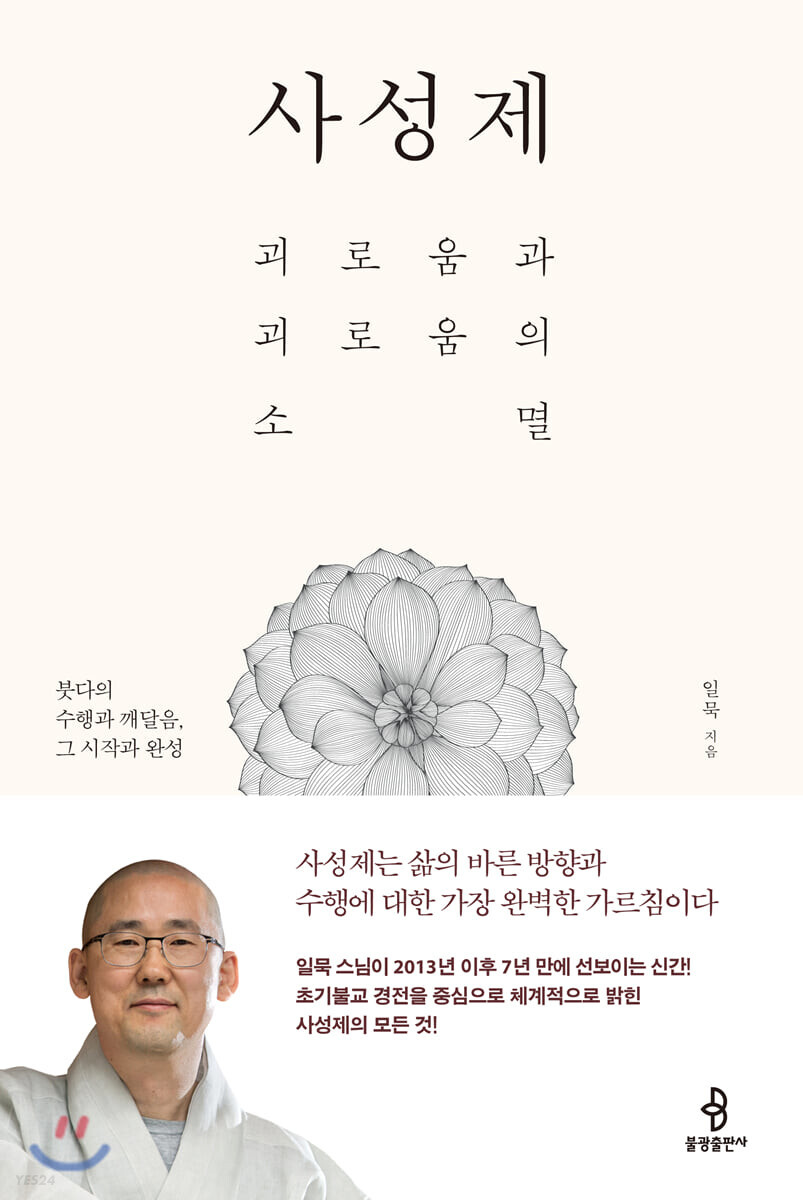
\includegraphics[width=0.6\columnwidth]{./fig/XL.jpg}
		\caption{	사성제 괴로움과 괴로움의 소멸 , 일묵 저, 불광출판사, 2020년 03월 24일}
		\label{fig:figure1}
		\end{figure}

	% ------------------------------------------ section ------------ 저자
	\newpage  \null
	\section{저자}

		\subsection{이력}
해인사 백련암에서 성철 큰스님의 제자인 원택 스님을 스승으로 모셨다. 
이후 범어사 강원을 졸업했고 봉암사, 미얀마 파욱국제명상센터, 영국 아마라와띠, 프랑스 플럼빌리지 등 국내외 수행처에서 수행하였다. 
2009년 서울에 초기불교 가르침을 전하는 제따와나선원을 개원하였고, 2018년 강원도 춘천으로 수행 도량을 이전하였다. 
현재 춘천 제따와나선원 선원장으로 있다. 

		\subsection{저서}

저서로 『이해하고 내려놓기』, 『일묵 스님이 들려주는 초기불교 윤회 이야기』, 『사성제』 등이 있다.

		\subsection{『이해하고 내려놓기』}
		\subsection{『일묵 스님이 들려주는 초기불교 윤회 이야기』}
		\subsection{ 『사성제』}



	% ------------------------------------------ section ------------ 
	\newpage  \null
	\section{목차}

\begin{quotation}

목차\\
서문\\
들어가며  붓다의 수행 여정과 깨달음\\

1장. 괴로움과 행복\\
1. 세속의 괴로움과 행복\\
1) 세속의 괴로움과 행복은 느낌이다\\
2) 괴로운 느낌이 괴로움이다
3) 행복한 느낌이 행복이다

2. 붓다의 괴로움과 행복\\
1) 붓다의 괴로움과 행복은 느낌이 아니라 특성이다
2) 괴로운 느낌은 괴로움이다
3) 행복한 느낌도 괴로움이다
4) 느낌은 괴로움이고, 느낌의 소멸이 행복이다

3. 괴로움과 행복에 대한 견해의 전환\\
1) 그릇된 견해와 바른 견해
2) 괴로움과 행복에 대한 진리의 가르침이 사성제이다

2장. 법이란 무엇인가?\\

1. 법이란 무엇인가?\\
1) 현상과 개념은 함께한다
2) 법은 붓다의 견해로 현상을 본 것이다
3) 존재의 실상은 물질과 정신의 법이다
4) 법을 괴로움과 괴로움의 소멸의 구조로 정리한 것이 사성제이다

2. 법에 대한 바른 이해\\
1) 법을 통해 법을 볼 수 있다
2) 법은 현상과 개념을 함께 나타낸다
3) 법은 현상보다 통찰이 중요하다
4) 개념에만 빠지지 말고 현상을 관찰해야 한다
5) 법은 스스로 보아 알 수 있다

3. 법을 알고 보면 괴로움이 소멸한다\\
1) 붓다의 견해는 사성제의 견해이다
2) 사성제의 견해를 통해 법을 본다
3) 법을 보면 사성제를 알 수 있다
4) 법을 알고 보면 괴로움이 소멸한다

3장. 연기\\

1. 연기\\
1) 연기
2) 연기된 법
3) 십이연기

2. 십이연기의 해설\\
1) 늙음·죽음은 태어남을 조건으로 일어난다
2) 태어남은 존재를 조건으로 일어난다
3) 존재는 취착을 조건으로 일어난다
4) 취착은 갈애를 조건으로 일어난다
5) 갈애는 느낌을 조건으로 일어난다
6) 느낌은 접촉을 조건으로 일어난다
7) 접촉은 여섯 감각 장소를 조건으로 일어난다
8) 여섯 감각 장소는 정신·물질을 조건으로 일어난다
9) 정신·물질은 의식을 조건으로 일어난다
10) 의식은 의도적 행위를 조건으로 일어난다
11) 의도적 행위는 무명을 조건으로 일어난다
12) 십이연기의 일어남과 소멸

3. 십이연기의 의미\\
1) 십이연기의 구조
2) 존재란 무엇인가?
3) 존재는 어떻게 태어났으며, 존재가 죽으면 어디로 가는가?

4. 연기는 중간의 가르침이다\\
1) 상견과 단견
2) 연기는 중간의 가르침이다
3) 연기와 사성제

4장. 사성제\\

1. 불교는 사성제이다\\
1) 불교는 괴로움과 괴로움의 소멸에 대한 가르침이다
2) 사성제는 진리의 가르침이다

2. 고성제: 괴로움의 성스러운 진리\\
1) 존재의 실상은 다섯 무더기이다
2) 다섯 무더기는 무상하고 괴로움이며 무아이다
3) 고성제: 다섯 무더기 자체가 괴로움이다
4) 고성제는 철저히 알아야 할 진리이다

3. 집성제: 괴로움의 일어남의 진리\\
1) 대상이 아니라 마음이다
2) 집성제: 갈애를 조건으로 괴로움이 일어난다
3) 해로운 법을 조건으로 괴로움이 일어난다
4) 집성제는 버려야 할 진리이다

4. 멸성제: 괴로움의 소멸의 진리\\
1) 멸성제: 갈애가 소멸하면 괴로움이 소멸한다
2) 해로운 법이 소멸하면 괴로움이 소멸한다
3) 열반과 단견의 차이
4) 아라한이 죽으면 어떻게 되는가?
5) 멸성제는 실현해야 할 진리이다

5. 도성제: 괴로움의 소멸로 인도하는 도 닦음의 진리\\
1) 도성제: 팔정도는 괴로움의 소멸로 인도한다
① 바른 견해
② 바른 사유
③ 바른 말
④ 바른 행위
⑤ 바른 생계
⑥ 바른 정진
⑦ 바른 기억
⑧ 바른 삼매
2) 유익한 법은 괴로움의 소멸로 인도한다
3) 도성제는 계발해야 할 진리이다

5장. 사성제에 대한 기억 확립\\

1. 불교의 수행은 중도 수행이다\\
1) 팔정도의 시작과 중간과 끝은 바른 견해이다
2) 팔정도는 계를 기반으로 정과 혜를 닦는 수행이다
3) 팔정도는 지관쌍수이다
4) 팔정도는 중도이다
5) 불교의 수행은 중도 수행이다

2. 중도 수행을 통해 사성제에 대한 기억이 확립된다\\
1) 중도 수행을 통해 사성제에 대한 기억이 확립된다
2) 사성제에 대한 기억 확립의 과정
3) 사성제에 대한 기억 확립이 깨달음이다
4) 아라한의 마음

나가며  가능한 일과 불가능한 일\\
참고문헌\\

\end{quotation}



\part{내용}


% ================================================= chapter 	====================
	\newpage
	\chapter{사성제 }


	% -------------------------------------- page -------------------
	%	\nomtcrule         		% removes rules = horizontal lines
	%	\nomtcpagenumbers  % remove page numbers from minitocs
		\newpage
		\minitoc				% Creating an actual minitoc
	%	\doublespace



	% ------------------------------------------ section ------------ 
	\newpage  \null
	\section{목차}

	% ------------------------------------------ section ------------ 
	\newpage  \null
	\section{서문}

	% ------------------------------------------ section ------------ 
	\newpage  \null
	\section{들어가며  붓다의 수행 여정과 깨달음}


% ===== ===== ===== ===== ===== ===== ===== ===== ===== ===== ===== ===== ===== ===== part
	\part{1장. 괴로움과 행복}

% ================================================= chapter 	====================
	\newpage

	\chapter{1. 세속의 괴로움과 행복}
	% -------------------------------------- page -------------------
	%	\nomtcrule         		% removes rules = horizontal lines
	%	\nomtcpagenumbers  % remove page numbers from minitocs
		\newpage
		\minitoc				% Creating an actual minitoc
	%	\doublespace


	% ------------------------------------------ section ------------ 
	\newpage  \null
	\section{1) 세속의 괴로움과 행복은 느낌이다}

	% ------------------------------------------ section ------------ 
	\newpage  \null
	\section{2) 괴로운 느낌이 괴로움이다}

	% ------------------------------------------ section ------------ 
	\newpage  \null
	\section{3) 행복한 느낌이 행복이다}

% ================================================= chapter 	====================
	\newpage
	\chapter{2. 붓다의 괴로움과 행복}
	% -------------------------------------- page -------------------
	%	\nomtcrule         		% removes rules = horizontal lines
	%	\nomtcpagenumbers  % remove page numbers from minitocs
		\newpage
		\minitoc				% Creating an actual minitoc
	%	\doublespace


	% ------------------------------------------ section ------------ 
	\newpage  \null
	\section{1) 붓다의 괴로움과 행복은 느낌이 아니라 특성이다}

	% ------------------------------------------ section ------------ 
	\newpage  \null
	\section{2) 괴로운 느낌은 괴로움이다}

	% ------------------------------------------ section ------------ 
	\newpage  \null
	\section{3) 행복한 느낌도 괴로움이다}

	% ------------------------------------------ section ------------ 
	\newpage  \null
	\section{4) 느낌은 괴로움이고, 느낌의 소멸이 행복이다}

% ================================================= chapter 	====================
	\newpage
	\chapter{3. 괴로움과 행복에 대한 견해의 전환}
	% -------------------------------------- page -------------------
	%	\nomtcrule         		% removes rules = horizontal lines
	%	\nomtcpagenumbers  % remove page numbers from minitocs
		\newpage
		\minitoc				% Creating an actual minitoc
	%	\doublespace

	\section{1) 그릇된 견해와 바른 견해}
	\section{2) 괴로움과 행복에 대한 진리의 가르침이 사성제이다}




% ===== ===== ===== ===== ===== ===== ===== ===== ===== ===== ===== ===== ===== ===== part
	\part{2장. 법이란 무엇인가?}


% ================================================= chapter 	====================
	\newpage
	\chapter{1. 법이란 무엇인가?}
	\section{1) 현상과 개념은 함께한다}
	\section{2) 법은 붓다의 견해로 현상을 본 것이다}
	\section{3) 존재의 실상은 물질과 정신의 법이다}
	\section{4) 법을 괴로움과 괴로움의 소멸의 구조로 정리한 것이 사성제이다}

% ================================================= chapter 	====================
	\newpage
	\chapter{2. 법에 대한 바른 이해}
	\section{1) 법을 통해 법을 볼 수 있다}
	\section{2) 법은 현상과 개념을 함께 나타낸다}
	\section{3) 법은 현상보다 통찰이 중요하다}
	\section{4) 개념에만 빠지지 말고 현상을 관찰해야 한다}
	\section{5) 법은 스스로 보아 알 수 있다}

% ================================================= chapter 	====================
	\newpage
	\chapter{3. 법을 알고 보면 괴로움이 소멸한다}
	\section{1) 붓다의 견해는 사성제의 견해이다}
	\section{2) 사성제의 견해를 통해 법을 본다}
	\section{3) 법을 보면 사성제를 알 수 있다}
	\section{4) 법을 알고 보면 괴로움이 소멸한다}



% ===== ===== ===== ===== ===== ===== ===== ===== ===== ===== ===== ===== ===== ===== part
	\part{3장. 연기}

% ================================================= chapter 	====================
	\newpage
	\chapter{1. 연기}
	\section{1) 연기}
	\section{2) 연기된 법}
	\section{3) 십이연기}

% ================================================= chapter 	====================
	\newpage
	\chapter{2. 십이연기의 해설}
	\section{1) 늙음·죽음은 태어남을 조건으로 일어난다}
	\section{2) 태어남은 존재를 조건으로 일어난다}
	\section{3) 존재는 취착을 조건으로 일어난다}
	\section{4) 취착은 갈애를 조건으로 일어난다}
	\section{5) 갈애는 느낌을 조건으로 일어난다}
	\section{6) 느낌은 접촉을 조건으로 일어난다}
	\section{7) 접촉은 여섯 감각 장소를 조건으로 일어난다}
	\section{8) 여섯 감각 장소는 정신·물질을 조건으로 일어난다}
	\section{9) 정신·물질은 의식을 조건으로 일어난다}
	\section{10) 의식은 의도적 행위를 조건으로 일어난다}
	\section{11) 의도적 행위는 무명을 조건으로 일어난다}
	\section{12) 십이연기의 일어남과 소멸}

% ================================================= chapter 	====================
	\newpage
	\chapter{3. 십이연기의 의미}
	\section{1) 십이연기의 구조}
	\section{2) 존재란 무엇인가?}
	\section{3) 존재는 어떻게 태어났으며, 존재가 죽으면 어디로 가는가?}

% ================================================= chapter 	====================
	\newpage
	\chapter{4. 연기는 중간의 가르침이다}
	\section{1) 상견과 단견}
	\section{2) 연기는 중간의 가르침이다}
	\section{3) 연기와 사성제}


% ===== ===== ===== ===== ===== ===== ===== ===== ===== ===== ===== ===== ===== ===== part
	\part{4장. 사성제}

% ================================================= chapter 	====================
	\newpage
	\chapter{1. 불교는 사성제이다}
	\section{1) 불교는 괴로움과 괴로움의 소멸에 대한 가르침이다}
	\section{2) 사성제는 진리의 가르침이다}

% ================================================= chapter 	====================
	\newpage
	\chapter{2. 고성제: 괴로움의 성스러운 진리}
	\section{1) 존재의 실상은 다섯 무더기이다}
	\section{2) 다섯 무더기는 무상하고 괴로움이며 무아이다}
	\section{3) 고성제: 다섯 무더기 자체가 괴로움이다}
	\section{4) 고성제는 철저히 알아야 할 진리이다}

% ================================================= chapter 	====================
	\newpage
	\chapter{3. 집성제: 괴로움의 일어남의 진리}
	\section{1) 대상이 아니라 마음이다}
	\section{2) 집성제: 갈애를 조건으로 괴로움이 일어난다}
	\section{3) 해로운 법을 조건으로 괴로움이 일어난다}
	\section{4) 집성제는 버려야 할 진리이다}

% ================================================= chapter 	====================
	\newpage
	\chapter{4. 멸성제: 괴로움의 소멸의 진리}
	\section{1) 멸성제: 갈애가 소멸하면 괴로움이 소멸한다}
	\section{2) 해로운 법이 소멸하면 괴로움이 소멸한다}
	\section{3) 열반과 단견의 차이}
	\section{4) 아라한이 죽으면 어떻게 되는가?}
	\section{5) 멸성제는 실현해야 할 진리이다}

% ================================================= chapter 	====================
	\newpage
	\chapter{5. 도성제: 괴로움의 소멸로 인도하는 도 닦음의 진리}
	\section{1) 도성제: 팔정도는 괴로움의 소멸로 인도한다}
① 바른 견해
② 바른 사유
③ 바른 말
④ 바른 행위
⑤ 바른 생계
⑥ 바른 정진
⑦ 바른 기억
⑧ 바른 삼매
	\section{2) 유익한 법은 괴로움의 소멸로 인도한다}
	\section{3) 도성제는 계발해야 할 진리이다}



% ===== ===== ===== ===== ===== ===== ===== ===== ===== ===== ===== ===== ===== ===== part
	\part{5장. 사성제에 대한 기억 확립}

% ================================================= chapter 	====================
	\newpage
	\chapter{1. 불교의 수행은 중도 수행이다}
	\section{1) 팔정도의 시작과 중간과 끝은 바른 견해이다}
	\section{2) 팔정도는 계를 기반으로 정과 혜를 닦는 수행이다}
	\section{3) 팔정도는 지관쌍수이다}
	\section{4) 팔정도는 중도이다}
	\section{5) 불교의 수행은 중도 수행이다}

% ================================================= chapter 	====================
	\newpage
	\chapter{2. 중도 수행을 통해 사성제에 대한 기억이 확립된다}
	\section{1) 중도 수행을 통해 사성제에 대한 기억이 확립된다}
	\section{2) 사성제에 대한 기억 확립의 과정}
	\section{3) 사성제에 대한 기억 확립이 깨달음이다}
	\section{4) 아라한의 마음}

% ===== ===== ===== ===== ===== ===== ===== ===== ===== ===== ===== ===== ===== ===== part
	\part{부록}	

	\section{나가며  가능한 일과 불가능한 일}
	\section{참고문헌}



% ------------------------------------------------------------------------------
% End document
% ------------------------------------------------------------------------------
\end{document}


